%----------------------------------------------------------------------------------------
%	7./ Opacity derivation
%----------------------------------------------------------------------------------------
%\section{Opacity derivation}
%\label{se:opacity}

The atmospheric opacity constitutes the ultimate limitation of
ground-based experiments. Only a fraction of the source 
signal is transmitted by the atmosphere and reaches NIKA2 detectors. 
The relation between the observed flux density
$\tilde{S}_{\nu}$ and the top-of-the-atmosphere flux density $S_{\nu}$
is parametrized by the zenith opacity $\taunu$
and the \airmass\ $x$ as %$x = \left(\sin\elev\right)^{-1}$, such as
\begin{equation}
\tilde{S}_{\nu} = S_{\nu} \, e^{-\taunu  x}.
\label{eq:uncorr_flux}
\end{equation}

An accurate derivation of the atmospheric opacity for each scan is
of outmost importance to retrieve the source signal and thus, to
ensure small calibration uncertainties.
%Opacity correction uncertainties even prevail in the
%final calibration error budget.
We developed three atmospheric opacity derivation methods, which are described in
Sect.~\ref{se:opacity_methods}. In Sect.~\ref{se:opacity_tests}, we
present robustness tests.
%extensively tested their
%robustness against observing conditions, as presented in
%Sect.~\ref{se:opacity_tests}.

\subsection{Atmospheric opacity estimation}
\label{se:opacity_methods}

%To assess the robustness of our opacity measurements,
We have developed three procedures for the atmospheric opacity
derivation: i) {\tt taumeter} relies on measurements
provided by the resident IRAM \taumeter\ operated at $225\,\rm{GHz}$;
%and a fit of the opacity estimates in NIKA2 frequency bands by imposing
%the flux density stability against atmospheric conditions;
ii) {\tt skydip} consists in using NIKA2 as a total-power \taumeter\ 
%(assuming the resonance frequencies are
%linearly related to the total power)
by resorting to a series of {\tt skydip} scans;
iii) {\tt corrected skydip} is a modified
version of the {\tt skydip} method that minimizes the dependence of the
estimated flux density on the opacity.

All methods i) do not rely on an ATM model nor on any
hypothesis on the atmospheric contents for the sake of robustness, and
ii) do not use the laboratory measurements of the bandpass (see 
Sect.~\ref{se:instru_bandpass}) for more accuracy.  

Sect~\ref{se:taumeter-method} presents the {\tt taumeter} method. The 
{\tt skydip} method is described in Sect~\ref{se:skydip-method} and
the selection of the used {\tt skydip} scans is discussed in
Sect.~\ref{se:skydip-selection}.
{\tt corrected skydip} is presented in Sect.~\ref{se:corrected-skydip}.

\subsubsection{The {\tt taumeter} method}
\label{se:taumeter-method}

The IRAM \trentemetre\ telescope facility is equipped with a
resident \taumeter\ operated at 225\,GHz. Every four
minutes, it performs elevation scans at fixed azimuth
to monitor the atmospheric opacity.
The IRAM science support
team provides us with time-stamped zenith opacities at $225\,\rm{GHz}$
$\tau_{225}$, as derived from the \taumeter\ measurements. The
$\tau_{225}$ estimates come in two different flavours: one relying
on a linear model and the other on an exponential fitting model. They
are then filtered by removing outliers and by thresholding on
goodness-of-fit criteria.
%$0< \tau_{225} <1.2$ and $R^2 > 0.99$, where $R^2$ is the coefficient
%of multiple determination of the $\tau_{225}$
%estimates, which quantifies the goodness of fit of each model.
%Redundant samples and outliers are removed.
Based on IRAM experience, we use the linear fit and filtered $\tau_{225}$
data for the NIKA2 analysis. The time-stamped $\tau_{225}$ estimates,
which are sampled about every 4 minutes, are interpolated to the time
of the NIKA2 scans (we consider the time of the middle of the
scan). For cross-check we also produce a smooth version of time-stamped
$\tau_{225}$ data by
filtering with a running median of seven samples, which is then
interpolated to the NIKA2 scan times.

We fit the relations between the IRAM
$225\,\rm{GHz}$ \taumeter\ opacities and NIKA2 band pass opacities using
observation of calibration sources which spans a large range of air
masses. This method has the advantages of not relying on atmospheric
model nor on the bandpass measurements in laboratory.
We use a series of 64 scans of MWC349, which consists of the
\baseline selected subset of scans from the 68 available scans for
this source during N2R9.
It constitutes an homogeneous data set in flux density but
heterogeneous in atmospheric conditions: zenith opacities at
$225\,\rm{GHz}$ range from 0.08 to 0.32 and elevations from $23$ to $73$
degrees, spanning a large range of \airmass\ as required.
NIKA2 opacities $\taunu$, for $\nu$ corresponding to the observing
frequency of Array 1, 2, 3 and the combination of Arrays 1 and 3, are estimated
from the $225\,\rm{GHz}$ \taumeter\ median-filtered linear-based opacity
estimates $\tau_{225}$ as
\begin{equation}  
  \tau_\nu =  a_\nu^{225}\tau_{225} + b_\nu^{225}.          
\end{equation}
The parameters $a_\nu^{225}$ and $b_\nu^{225}$ are fitted
to the data set so that the source flux density %to ensure
%that the non-corrected flux densities $\tilde{S}_\nu$ are stable against
%$\tau_{225}$ after correction of the atmospheric attenuation by
%inversion of Eq.~\ref{eq:uncorr_flux} using 
\begin{equation}  
  S_\nu = \tilde{S}_\nu\,\, e^{(a_\nu^{225}\tau_{225} + b_\nu^{225}) \, x}, 
  \label{eq:opacorr_taumeter}
\end{equation}
is constant within scans.

\begin{table}[!htbp]
  \begin{center}
    \caption[IRAM \taumeter\ to NIKA2 opacity model]{{\lp Best-fit
    parameters and rms uncertainties to infer NIKA2 opacities from the IRAM \taumeter\ measurements.}}
    \label{tab:tau225-to-taunika}  
    \begin{tabular}{lrrrr}
      \hline
      \hline
      \noalign{\smallskip}
      Parameters & Array 1 & Array 3  & Array 1$\&$3 & Array 2  \\
      \noalign{\smallskip}
      \hline
      \noalign{\smallskip}
      $a_\nu^{225}$         & $1.94$   &  $1.90$ &  $1.92$ & $0.94$ \\
      $b_\nu^{225}$         & $-0.04$  & $-0.07$ & $-0.06$ & $0.00$ \\
      $\Delta a_\nu^{225}$  & $0.15$  & $0.08$  &  $0.09$ & $0.10$ \\
      $\Delta b_\nu^{225}$  & $0.05$  & $0.03$  & $0.04$ & $0.03$ \\
      \noalign{\smallskip}
      \hline
    \end{tabular}
  \end{center}    
\end{table}

We tested two estimators of the flux stability. The first one relies
on minimizing the standard deviation of the measured-to-median flux
densities ratio after atmospheric opacity correction using
Eq.~\ref{eq:opacorr_taumeter}. The second one is obtained by minimizing
\begin{equation}
\chi^2 = \sum_{i=1}^{N} \frac{1}{\sigma^2} \, \left( \frac{S_\nu}{\rm{Med}(S_\nu)} -1 \right)^2,  
\end{equation}
where $\sigma$ is the rms uncertainty of the flux density estimates. Note
that these estimators do not depend on
the absolute scale of the flux density of the source. Both estimators
yield consistent results that are combined and gathered in
Table.~\ref{tab:tau225-to-taunika}. The quoted errors
$\Delta a_\nu^{225}$ and $\Delta b_\nu^{225}$ are 1-$\sigma$ errors of
the fit.

Because the IRAM \taumeter\ observes at a fixed azimuth, the
{\tt taumeter} opacities are not the line-of-sight opacities
for the observation scans. As this will be verified in
Sect.~\ref{se:photometry}, this induces larger rms errors of
the top-of-the-atmosphere flux density estimates compared to
opacity correction methods that relies on NIKA2 skydip-based
measurements. The {\tt taumeter} method will thus be used
as an alternative method in case of failure of the NIKA2 skydip-based
methods and to perform consistency checks.


\subsubsection{NIKA2 skydip-based method}
\label{se:skydip-method}

The NIKA2 {\tt skydip} method for the opacity derivation consists in
using the NIKA2 instrument as an in-band total-power \taumeter. {\lp The opacity
integrated in the NIKA2 bandpasses and in the line-of-sight of the
observing scan is thereby directly obtained.} 
This idea,
which was successfully tested with NIKA~\citep{Catalano2014}, relies
on the fact that the resonance frequency of each KID varies linearly
with the total power, as discussed in Sect.~\ref{se:tuning}.
First, we have to calibrate the relationship between total
power and opacity. Then, we can use this calibration to measure the
opacity during a given scan. %Using this procedure we thus directly
%derive an opacity integrated in the NIKA2 bandpasses and in the
%line-of-sight of the observing scan.

First, we detail the opacity calibration. For each KID $k$, the
absolute value of its resonance frequency $f_{\rm{reso}}^k$ varies with the
atmospheric load according to
%
\begin{equation}
f_{\rm{reso}}^k  = c_0^k - c_1^k T_{\rm{atm}}[1-e^{-\taunu x}]
\label{eq:skydip}
\end{equation}
%
where $c_0^k$ is a constant equal to the KID resonance frequency at zero
opacity, $c_1^k$ is a calibration conversion factor in Hz$/$K,
$T_{\rm{atm}}$ is the temperature of the atmosphere. %, $\taunu$ the zenith
%opacity and $\elev$ the observing elevation.
By assuming a homogeneous plane-parallel atmosphere, the
\airmass\ $x$ is defined from the elevation as
$x = \left(\sin\elev\right)^{-1}$. {\lp The Earth sphericity can be safely
neglected at the elevations under discussion here.}
We take $T_{\rm{atm}}$ as a constant equal to 270\,K. However, the opacity is
expected to slightly depend on the atmospheric temperature. For
example, in poor weather conditions (6\,mm of water vapor contents),
the zenith opacity in {\lp both observing bands} can vary by
about 10\% for temperature variations of 10\,K. The
effect of the temperature variations on the final
calibration of NIKA2 response to the sky load is mitigated by using
several dedicated observation scans regularly distributed all along an
observation campaign.

%%%%%%%FIG8
The $c_0^k$ and $c_1^k$ are determined using {\tt skydip} scans, which
consist in moving the telescope in elevation step by step, as
defined in Sect.~\ref{se:skydip}. For each KID $k$, the evolution
of $f_{\rm{reso}}^k$ is monitored as a function of the \airmass\ in each
elevation step to perform a joint fit of the zenith opacity $\taunu$ and
the $c_0^k$ and $c_1^k$ coefficients.
%The acquisition time spent on each elevation step, which is of about
%twenty seconds, is chosen to reduce the error in the determination of
%$f_{reso}$.
All skydips, obtained under various opacity conditions, are analysed
together to break the degeneracy between the opacity and the
Herz-to-Kelvin conversion factor $c_1^k$. The degeneracy occurs mostly for low opacity
conditions for which we can only determine the combination
$c_1^k \taunu x$. The procedure has two steps. First, all the {\tt
skydip} scans are analysed individually to extract $f_{\rm{reso}}^k$ for each
stable elevation and for each KID. Secondly, a simultaneous fit is done
for all parameters (one $\taunu$ per skydip, and a set of $c_0^k$ and
$c_1^k$ for all KIDs). Figure~\ref{fig:skydipfitexample} illustrates the
fitting procedure.
%
\begin{figure}[!htbp]
\begin{center}
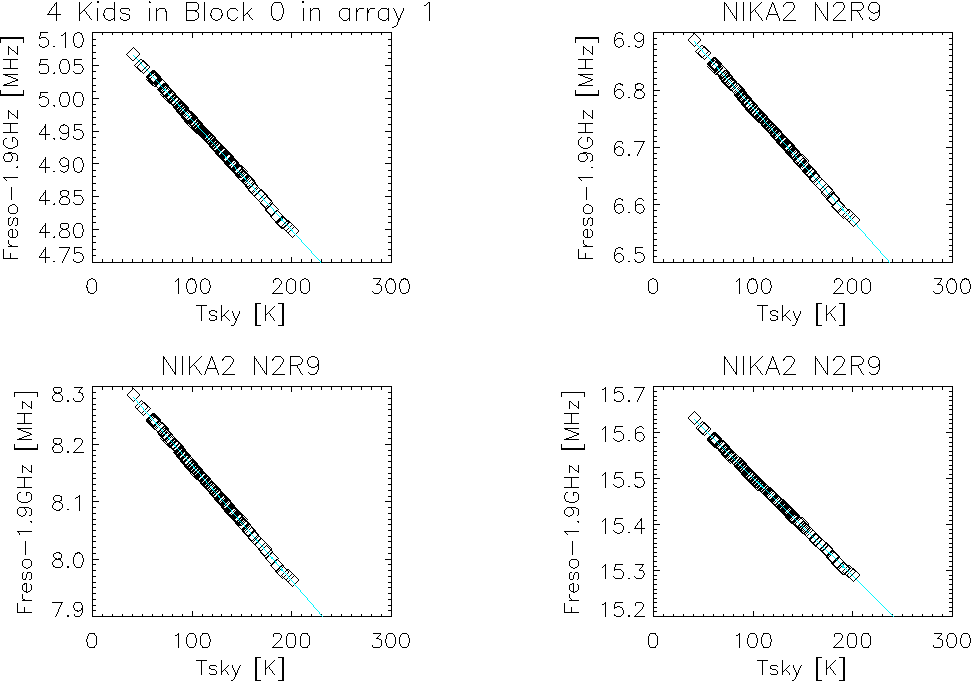
\includegraphics[trim={9cm 0cm 0cm 6.5cm}, clip=true, width=0.9\linewidth]{Figures/test_allskd4_N2R9v5_5-crop.pdf}
\caption[]{Example of the global skydip fit for a KID.
Each square point represents one step in a skydip (made of eleven
elevation steps). A series of 12 {\tt skydip} scans are jointly used
spanning zenith opacities from 0.15 to 0.50 {\lp in the $1\,\rm{mm}$ band}. The horizontal axis gives the sky
effective temperature $T_{\rm{sky}} = T_{\rm{atm}}[1-e^{-\taunu\, x}]$ in Kelvin, where $\taunu$ is the
skydip zenith opacity found in the fit. The vertical axis shows the relative
resonance frequency of the KID with respect to 1.9\,GHz, given in MHz. The blue line is the linear
model using the best-fit $c_0^k$ and $c_1^k$ coefficients (see
Eq.~\ref{eq:skydip}).}
\label{fig:skydipfitexample}
\end{center}
\end{figure}
%
{\lp This fit is performed on block of 40 KIDs. We check that the
resulting $\taunu$ from the different blocks are consistent within rms
errors, which are equal to about $4\times 10^{-3}$ at 1\,mm and
$1\times 10^{-3}$ at 2\,mm.}
%Uncertainties on $\taunu$ are estimated by doing this
%procedure on blocks of 40 KIDs only and getting a dispersion on the resulting
%$\taunu$ from the different blocks. Usually the dispersion comes out as
%$4\times 10^{-3}$ at 1\,mm and $1\times 10^{-3}$ at 2\,mm.
Once the $\taunu$ values are estimated for each {\tt skydip} (as the average over the
blocks), we compute, while fixing the $\taunu$, the $c_0^k$ and $c_1^k$
final values for each KID $k$ with a linear fit. We thus retrieve
the coefficients of all the KIDs even though some of them could not
contribute to the $\taunu$ determination. %We find that the skydip-fitted
%$\taunu$ values are, as expected, consistent between different detectors of
%the same array.

{\lp We have observed that the  $c_0^k$ and $c_1^k$ coefficients vary
between observational campaigns due to a change in the KID properties
from one cooldown to another.}
However, by comparing the results of different skydips, we have verified that the
coefficients $c_0^k$ and $c_1^k$ are stable, within the fitting errors, on very
long time scales within a cooldown cycle. The coefficients can thus be
applied to the whole observing campaign for the opacity derivation. % in order to recover the
% opacity of each scan.
Specifically, the opacity %for each array
%$A_i$, $i=\{1, 2, 3\}$
is retrieved for each observation scan by
inverting Eq.~\ref{eq:skydip} as:
\begin{equation}
\taunu =   \rm{Med}\left( -\frac{1}{x} \log\left( \frac{f_{\rm{reso}}^k - c_0^k}{c_1^kT_{\rm{atm}}} +1 \right)\right), 
\end{equation}
%where $\nu$ stands for the observing frequency of array A1, A2, A3 or the array
%combination A1$\&$A3, and
where the median is evaluated using all the valid
KIDs of the arrays under concern. Hence, we are able to derive an opacity
integrated in the NIKA2 bandpasses and in the line-of-sight of the
source in the considered observation scan.

\subsubsection{{\tt Skydip} scan selection}
\label{se:skydip-selection}

The {\tt skydip} opacity derivation requires to have on hands a
sizeable amount of {\tt skydip} scans --
typically ten to twenty -- that i) span the whole opacity range and
ii) avoid highly perturbed atmosphere to meet the plane-parallel
atmosphere assumption. To that aim, we perform a {\tt skydip}
scan twice a day during a scientific campaign. Then, the ($c_0^k$, $c_1^k$)
determination process relies on a selection of the {\tt skydip} scans.
%%%%%%% FIG9
%%%%%%% FIG10

%\begin{figure}[!htbp]
%  \begin{center}
%    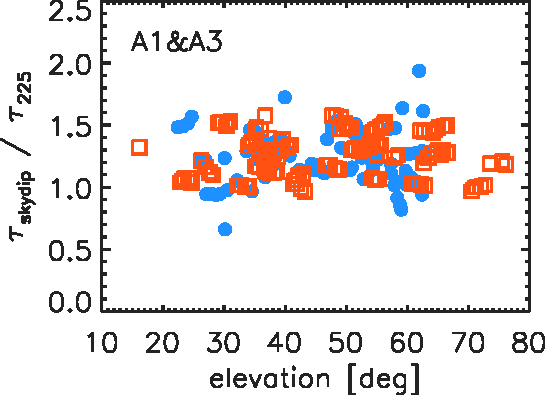
\includegraphics[clip=true, trim={0, -0.3cm, -0.3cm, 0}, width=0.42\textwidth]{Figures/Opacity_skydip_to_taumeter_vs_elev_1mm.pdf}
%    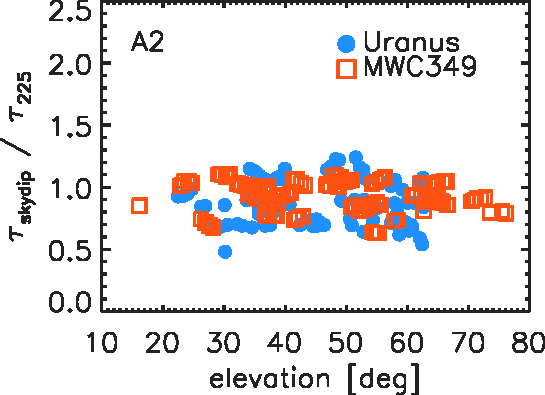
\includegraphics[clip=true, trim={0, -0.3cm, -0.3cm, 0}, width=0.42\textwidth]{Figures/Opacity_skydip_to_taumeter_vs_elev_a2.pdf}
%    \caption[NIKA2 skydip-based opacity stability against observing elevations]{NIKA2
%    skydip-based opacities stability against the observing
%    elevation. The ratio between the skydip-based opacities and the
%    taumeter-derived opacities is shown as a function of the observing
%    elevation as blue points for Uranus scans and empty red square for
%    MWC349 scans. See discussion in Sect.~\ref{se:opacity_tests}.} 
%\label{fig:skydip-to-taumeter-ratio-vs-elev}
%\end{center}
%\end{figure}

For each {\tt skydip} scan and %for each block of 40 KIDs,
for each KID, 
we compute the difference between the measured KID resonance frequency and the model
given in Eq.~\ref{eq:skydip} taken at the best-fit values of the
($c_0^k$, $c_1^k$) parameters{\lp, which is named $df_{\rm{reso}}^k$.} Then, we
determine two indicators of the fit quality per {\tt skydip}. {\lp First,
for each block of 40 KIDs, the standard deviation of $df_{\rm{reso}}^k$ is calculated
over all the KIDs of the block. This standard deviation per KID block
is called $\sigma_{40}$. For each {\tt skydip}, we evaluate the
median rms, which is the median $\sigma_{40}$ over all the KID blocks.} 
%, given in Hz.
%
\begin{figure}[!htbp]
\begin{center}
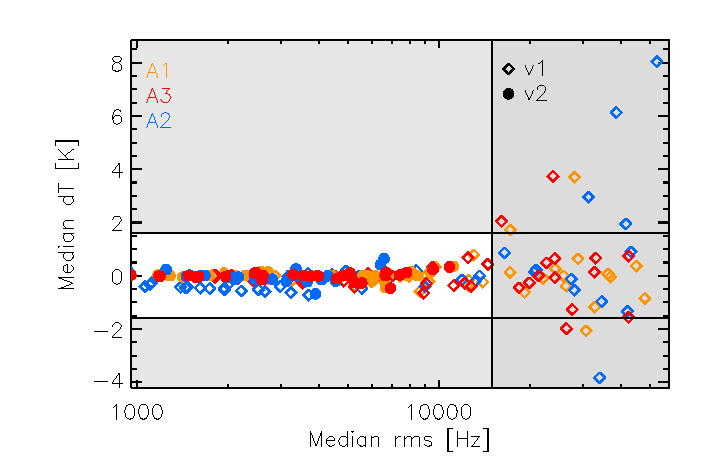
\includegraphics[clip=true,width=\linewidth]{Figures/plot_skydip_selection_two_crit.pdf}
\caption[N2R9 skydip scan selection.]{ Median dT quality-fit criterion
is plotted as a function of the median rms criterion for each skydip
scan of the N2R9 campaign and for the three arrays. {\lp The {\tt
skydips} that yield a poor fit of the KID resonance frequencies and hence
do not met Median dT criterion, are also discarded using
Median rms. The latter criterion further discards noisy {\tt skydips}.}
%Both criteria are nicely correlated.
Empty diamonds show the results of the first
iteration of the skydip coefficient estimation, labeled 'v1', whereas
filled circles show the second iteration, labeled 'v2', for which only the skydips
that met both fit-quality criteria are included.
After the second iteration, all the remaining skydips met the criteria.}
\label{fig:skydipselection}
\end{center}
\end{figure}
%
This fit quality indicator is also sensitive to the noise
level during the {\tt skydip}. We therefore devise a second fit quality
indicator to further measure the bias between the data and the
best-fit model.
Namely, for each {\tt skydip}, we compute the average
$df_{\rm{reso}}^k$ of each KID $k$ and convert this quantity from Hertz to Kelvin
using the corresponding $c_1^k$ parameter. This cross-calibration
allows us to compare the $df_{\rm{reso}}^k$ estimates from different KIDs.
Median $dT$ is the median of the average $df_{\rm{reso}}^k$ in Kelvin over all the KIDs of an
array. With these two indicators in hands, we discard the {\tt skydip} scans
that are noisy or that yield a poor fit by applying the following selection
criteria:

\begin{itemize}
\item Median $\rm{rms} < 1.5 \times 10^{4}~\rm{Hz}$
\item Median $dT < 1.6~\rm{K}$
\end{itemize}

The threshold values have been determined using the set of 44 {\tt skydip}
scans of N2R9. The Median rms cut corresponds to twice the median of
this quantity per {\tt skydip} scan, whereas the Median $dT$ cut is twice
the standard deviation of Median $dT$ over the {\tt skydip} scans.
N2R9 {\tt skydip} scan selection is illustrated in
{\lp Fig.~\ref{fig:skydipselection},
which shows the complementarity between the two fit-quality
criteria. After selection, 15 skydips are kept for the final step of
the ($c_0^k$, $c_1^k$) fit in the case of the N2R9 campaign.}

The ($c_0^k$, $c_1^k$) estimation proceeds in two steps: first the
parameters are estimated using all the available {\tt skydip} scans for a
given campaign, then the estimation is repeated using only
{\tt skydip} scans that met the fit-quality criteria. After the second
iteration, we check that no extra {\tt skydip} scan outliers are left, as shown by
the 'v2' label data points in Fig.~\ref{fig:skydipselection}.
%After
%selection of the skydip scans acquired during the N2R9 campaign, 15
%skydips are kept for the final step of the ($c_0$, $c_1$) fit.
%
\begin{figure*}[!thbp]
  \begin{center}
    \begin{overpic}[clip=true, trim={0, -0.3cm, -0.3cm, 0}, width=0.3\textwidth]{Figures/Opacity_correl_skydip_vs_tau_a1.pdf}
      \put(0,70){\footnotesize a)}
    \end{overpic}
    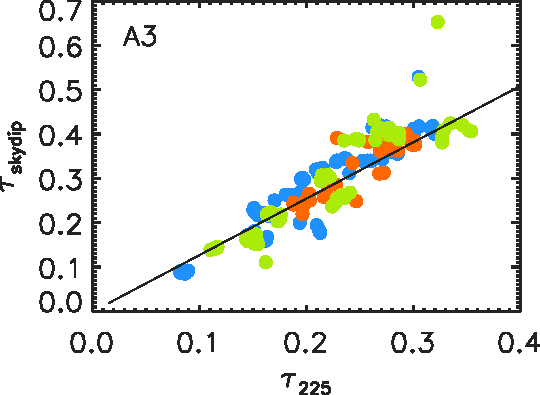
\includegraphics[clip=true, trim={0, -0.3cm, -0.3cm, 0}, width=0.3\textwidth]{Figures/Opacity_correl_skydip_vs_tau_a3.pdf}
    \begin{overpic}[clip=true, trim={-0.3cm, -0.3cm, 0, 0}, width=0.3\textwidth]{Figures/Opacity_skydip_to_taumeter_vs_elev_1mm.pdf}
      \put(0,70){\footnotesize b)}
    \end{overpic}
    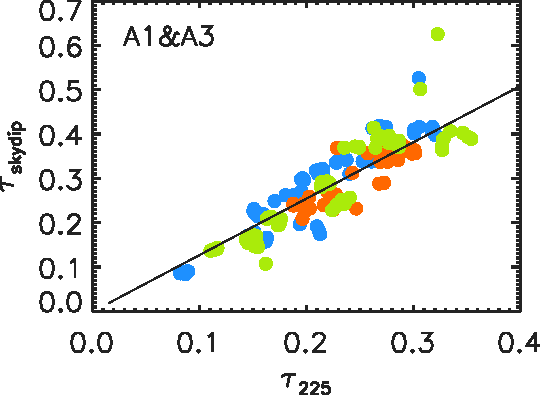
\includegraphics[clip=true, trim={0, -0.3cm, -0.3cm, 0}, width=0.3\textwidth]{Figures/Opacity_correl_skydip_vs_tau_1mm.pdf}
    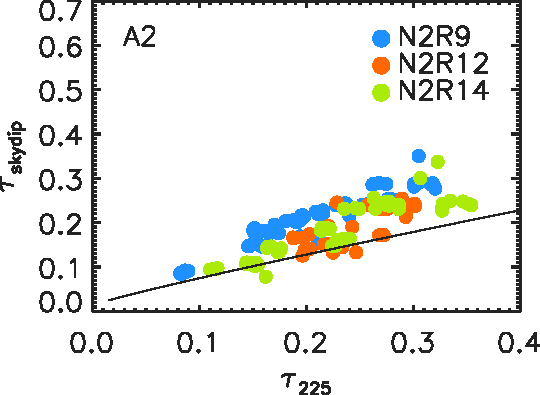
\includegraphics[clip=true, trim={0, -0.3cm, -0.3cm, 0}, width=0.3\textwidth]{Figures/Opacity_correl_skydip_vs_tau_a2.pdf}
    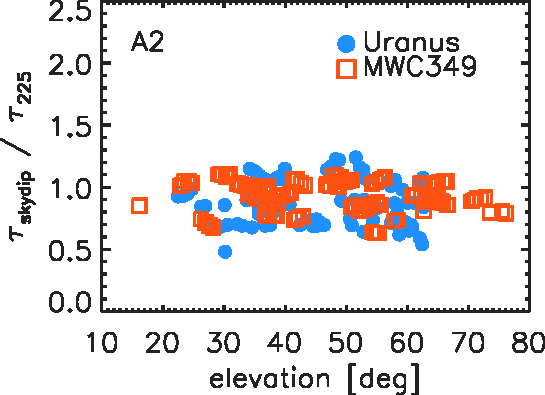
\includegraphics[clip=true, trim={-0.3cm, -0.3cm, 0, 0}, width=0.3\textwidth]{Figures/Opacity_skydip_to_taumeter_vs_elev_a2.pdf}
   \caption[]{NIKA2
     skydip-based opacities $\taunu^{\rm{skydip}}$ consistency checks.
     a) $\taunu^{\rm{skydip}}$ vs median-filtered
    time-stamped IRAM 225\,GHz \taumeter\ opacities (see
    Sect.~\ref{se:taumeter-method}).
    For illustration purpose, the modeled correlations relying on an ATM model integrated in
    NIKA2 frequency bands are shown in black. b) $\taunu^{\rm{skydip}}$ stability against the observing
    elevation. The ratio between the skydip-based opacities and the
    \taumeter-derived opacities is shown as a function of the observing
    elevation as blue points for Uranus scans and empty red square for
    MWC349 scans. See discussion in Sect.~\ref{se:opacity_tests}. } 
\label{fig:skydip-to-taumeter-correl}
\end{center}
\end{figure*}
%
The stability of the ($c_0^k$, $c_1^k$) parameters and hence the
{\tt skydip} opacity estimates, have been tested against the
choice of the selection criteria. We found that the $\taunu$
estimates are robust against the {\tt skydip}-scan selection as long as the
selection includes good {\tt skydip} scans in high opacity condition
$(\tau_{1\rm{mm}} > 0.44)$ and as the poor
fitting {\tt skydip} scans, which mostly correspond to deviation from the
atmosphere plane-parallel model in high opacity {\tt skydip} scans (as seen in
Fig.~\ref{fig:skydipselection}), are excluded.
%When these conditions
%are met, the {\tt skydip}-scans selection induces uncertainties on the zenith
%opacities that are below $10\%$ at 1\,mm and below $15\%$ at 2\,mm.  


\subsubsection{{\tt Corrected skydip}}
\label{se:corrected-skydip}
The opacity estimates are ultimately tested by assessing the
stability of the top-of-the-atmosphere flux densities of bright sources for a large
range of atmospheric conditions, as will be addressed in
Sect.~\ref{se:photometry}. After opacity correction using the
{\tt skydip} $\taunu$ estimate, the calibration flux density
measurements show a residual dependency on the atmospheric
transmission, as discussed in Sect.~\ref{se:photometry}. This has
motivated the development of a corrected version of the {\tt skydip}
method that ensures the robustness of the flux densities against
atmospheric conditions.

{\lp As already noticed in Sect.~\ref{se:skydip-method}, for small values of the
line-of-sight opacity $\taunu x$, only the parameter combination
$c_1^k T_{\rm{atm}}\taunu$ is constrained in
Eq.~\ref{eq:skydip}. Degeneracies between $c_1^k$ parameters, the
atmospheric temperature and $\taunu$ can translate into a
scaling factor in the fitted skydip opacities
$\taunu^{\rm{skydip}}$. To take this effect into account, }  
we use the flux stability estimators described in
Sect.~\ref{se:taumeter-method} to fit a correction to $\taunu^{\rm{skydip}}$ as
\begin{equation}  
  \taunu =  a_\nu^{\rm{skydip}}\taunu^{\rm{skydip}}.
  \label{eq:corrected_skydip}
\end{equation}

We find $a_\nu^{\rm{skydip}}$ of
$1.36 \pm 0.04$,
$1.23 \pm 0.02$,
$1.27 \pm 0.03$ and
$1.03 \pm 0.03$ for A1, A3, A1$\&$A3 and A2 respectively.
% a   = 1.3600000       1.0318470       1.2326556       1.2660000
% s_a = 0.038587182     0.028553570     0.019324699     0.026832816

Moreover, we test for an additional offset in the
correcting relation of the {\tt skydip} opacities given in
Eq.~\ref{eq:corrected_skydip}. We find best-fitting correcting factors
in agreement with the best-fit values estimated using the single-parameter
correcting relation, whereas the best-fit offsets are compatible with
zero at both wavelengths. We conclude that correcting the {\tt skydip}
opacity estimates for a normalisation as given in
Eq.~\ref{eq:corrected_skydip} suffices for ensuring flux density
robustness against atmospheric opacity conditions.

The exact physical origin for the discrepancy of the empirical factor
$a_\nu^{\rm{skydip}}$ from the expected unity value {\lp for the
$1\,\rm{mm}$ wavebands} is currently under investigation.
{\lp Beside the $c_1^k$-to-$\taunu$ degeneracy and the effect
of the variation of the atmospheric temperature, possible explanations
also include a ground pick-up effect. Indeed a fraction of the beam
detects radiation from the ground, as evidenced by forward
efficiency measurements using heterodyne front-ends (see
Sect.~\ref{se:beam_efficiency}).}
%First, the possible explanations include a deviation
%from the opacity-to-resonance model of Eq.~\ref{eq:skydip},
%, a limit in the validity of the underlying assumptions (e.g. plane-parallel atmosphere,
%constant temperature) or a ground pick-up effect.
However,
the stability of the flux densities corrected using the
{\tt corrected skydip} opacities {\lp and the results consistency using
several observation campaigns}, as discussed in
Sect.~\ref{se:photometry}, constitutes a validation of this approach.


\subsection{Opacity estimate consistency checks}
\label{se:opacity_tests}

First, we test the stability of the {\tt skydip} opacities from one
observation campaign to
another. Panels a) in Fig.~\ref{fig:skydip-to-taumeter-correl} show the
correlation between the {\tt skydip} $\taunu$ estimates $\taunu^{\rm{skydip}}$
and the median-filtered time-stamped IRAM $225\,\rm{GHz}$ \taumeter\ 
zenith opacities $\tau_{225}$, as described in
Sect.~\ref{se:taumeter-method}, for a series of scans
of Uranus and MWC349 acquired during the {\emph reference} observation
campaigns. As guidelines,
we also show the predicted correlations using an ATM model integrated
in the NIKA2 bandpasses and in the $225\,\rm{GHz}$ band. {\lp The
$\taunu^{\rm{skydip}}$ to $\tau_{225}$ correlation relations are
consistent within statistical errors for the three campaigns.}
At 1\,mm they are also in agreement with the ATM model expectations,
while at 2\,mm the ATM model underestimates the measured {\tt skydip}
$\taunu$. {\lp Using the correction described in
Sect.~\ref{se:corrected-skydip}, the ATM
model consistently underestimates the {\tt corrected skydip} opacity
estimates at both wavelengths.}
% tau_correctedskydip = 1.3 tau_225^ATM
%At 2\,mm, more
%dispersion is observed between each correlation relations although
%they are compatible with each others within statistical errors.
%We note that the ATM model underestimates the
%measured {\tt skydip} $\taunu$.
This mild discrepancy with the ATM model predictions is yet to be
understood, but has no impact on
our opacity measurements, which do not rely on this model nor on
the precision with which the observing bandpasses are known. {\lp
Further consistency test with ATM expectations will be performed in the
future using in-situ bandpass measurements with a
dedicated Martin-Pupplett spectrometer.}


We further check the robustness of $\taunu^{\rm{skydip}}$ against the
observing elevation. 
%Figure~\ref{fig:skydip-to-taumeter-ratio-vs-elev}
Panel b) in Fig.~\ref{fig:skydip-to-taumeter-correl} shows the ratio of NIKA2
{\tt skydip} opacities to the $225\,\rm{GHz}$ \taumeter\ opacities as a function of
the average scan elevation. The {\tt skydip} opacity measurements have
no significant dependency on the elevation. Moreover, we observe that
the results are consistent for Uranus \bm\ scans and for
the shorter raster scans of the secondary calibrator MWC39, indicating
that the {\tt skydip} opacity estimates do not depend on the type of
observation scans.


As a summary, NIKA2 {\tt skydip} opacity estimates i) have reproducible
correlation coefficients with the $225\,\rm{GHz}$ \taumeter\ opacities from a
campaign to another, ii) are robust against the observing conditions,
and iii) are stable for various sources and scanning strategies. {\lp
In addition to these properties, the {\tt corrected skydip} opacities
further ensure flux density measurements that are immune to the
atmospheric and observing elevation conditions. We use them in
the \emph{baseline} calibration.}


